\documentclass{article}
\usepackage[utf8]{inputenc}
\usepackage{amssymb,amsmath,graphicx,indentfirst}

\title{EP4 - MCMC}
\author{George Othon - NUSP 103xxxxx 
        \\ Felipe Zaffalon - NUSP 103xxxxx}
\date{Maio de 2020}

\begin{document}

\maketitle

\section{Introdução}

Este relatório tem como objetivo calcular uma aproximação para a seguinte integral:

\hfill

$$ \int_0 ^ {+\infty} h(x) g(x) dx $$

\hfill

\par Onde h(x) é função indicadora no intervalo [1,2]. Com h(x) = $ I( 1 \leq x \leq 2 )$. E g(x) $ \propto$ gamma(C,x).$\left|\cos (Rx)\right|$, ou seja, g(x) = k.gamma(C,x).$\left|\cos (Rx)\right|$, com k $\in \mathbb{R}$. Com os parâmetros C = 1.39xxxxxxx e R = 1.103xxxxx.

\par A aproximação será feita através de dois algoritmos, o de Metropolis e o de Baker, em que os dois utilizam a cadeia de Markov, e a única diferença é o parâmetro de aceitação.

\section{Resultados}
Para gerar uma aproximação, criamos duas funções no python, uma que utiliza o algoritmo de Metropolis e outra por Baker. A condição de parada foi quando o erro atingisse 1\% ou menos, a partir de um número mínimo de passos.

\par Como resultado obtivemos que:

\hfill

\begin{figure}[!htb]
    \centering
    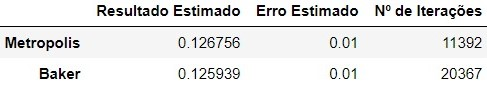
\includegraphics[scale=0.8]{Tabela1.jpeg}
    \caption{Resultados}
    \label{fig:my_label}
\end{figure}

\par Para chegar neste erro estimado utilizamos a seguinte métrica:
$$ erro = \frac{\sigma}{\sqrt{N}} $$

% quando aplicada a função h(x)

\hfill

\par Em que $\sigma$ é o desvio padrão da cadeia de Markov, e N o tamanho da cadeia.



\par Para calcular a função g não foi necessário saber o k, já que, tanto na aceitação alpha de Metropolis quanto na de Baker calculamos uma razão que cancela o multiplicador k. 
\par Para o algoritmo de Metropolis:

%Equação de Metropolis

\begin{equation*} %\label{eq1}
    \begin{split}
        alpha & = \frac{g(x_n)}{g(x_{n-1})}\\
            & =  \frac{k.gamma(C,x_n).\left|\cos (Rx_n)\right|}{k.gamma(C,x_{n-1}).\left|\cos (Rx_{n-1})\right|}\\
            & = \frac{gamma(C,x_n).\left|\cos (Rx_n)\right|}{gamma(C,x_{n-1}).\left|\cos (Rx_{n-1})\right|}
    \end{split}
\end{equation*}

\hfill

\par E para o algoritmo de Baker, temos:

%Equação de Baker

\begin{equation*} %\label{eq1}
    \begin{split}
        alpha & = \frac{g(x_n)}{g(x_{n-1}) + g(x_{n})}\\
            & =  \frac{k.gamma(C,x_n).\left|\cos (Rx_n)\right|}{k.gamma(C,x_{n-1}).\left|\cos (Rx_{n-1})\right| + k.gamma(C,x_n).\left|\cos (Rx_n)\right|}\\
            & = \frac{gamma(C,x_n).\left|\cos (Rx_n)\right|}{gamma(C,x_{n-1}).\left|\cos (Rx_{n-1})\right| + gamma(C,x_n).\left|\cos (Rx_n)\right|}
    \end{split}
\end{equation*}

\hfill

\par Logo, não é necessário saber o k para calcular essa integral pelo método MCMC.

\hfill

\par Após diversos testes percebemos que com o aumento do desvio padrão, a quantidade de passos até atingir o erro esperado era maior, e quando o desvio padrão era muito próximo de zero não tinhamos uma boa aproximação.

\hfill

\par Para não permitir valores de x negativos, nós colocamos ele em módulo. Isso é possível pois, por estarmos usando uma curva normal centrada no zero para gerar o número aleatório, temos que a probabilidade de um valor ser negativo é a mesma de seu oposto. Logo, não estamos alterando a aleatoriedade do gerador.


\hfill

\par Para encontrar o número adequado de passos para obter erro menor ou igual a 1\%, a partir de 2000 iterações passamos a calcular o erro e verificar se atendia ao requisito, e enquanto não atendesse nós incrementamos o número de passos.



\end{document}
